\chapter{Two-Dimensional Radiative Transfer}

% \begin{itemize}
%     \item Adding a dimension to RT, formal solver etc.
%     \item Simulation setup.
%     \item Analysis.
%     \item Suggestions on visibility of this chromospheric glow with DKIST.
% \end{itemize}

All of the theory of radiative transfer discussed in previous chapters remains valid when applied to higher dimensional systems, with the exception of the formal solver.
This is due to the non-local terms that appear within the MALI description (with diagonal $\Lambda$ operator) being handled by formal solver, which is responsible for computing the radiation field throughout the plasma from the local parameters and boundary conditions and thus coupling the atmospheric nodes.
Once the radiation field has been computed it is then used as a local parameter in the rest of the iteration.
In fact, if the storage for the atmosphere is ``flattened'' into a one-dimensional form, the code from the plane-parallel case can be used to implement the iteration scheme.

In this chapter we shall first describe the extension of the \Lw{} framework to two dimensions (with the possibility of further extension), and then describe its application to the simulation of a flaring atmosphere illuminating an adjacent slab of quiet sun, along with potential implications for future observations at high resolution.

\section{The Formal Solver in Two-Dimensions}

Similarly to the plane-parallel formal solver used in \Lw{}, described in the previous chapter, we use the short-characteristics method to compute the radiation field throughout the atmosphere.
This approach was first employed in two-dimensions by \citet{Auer1994} using a limited parabolic scheme to avoid overshoot.
We assume the following basis: the $z$-axis is oriented as in the plane-parallel case, oriented vertically from photosphere to corona, the $x$-axis is perpendicular and co-planar to the $z$-axis (in the plane of the page for the following diagrams), and by the right-hand rule the $y$-axis is oriented into the plane of the page.
In the two-dimensional case it is assumed that the atmospheric parameters are homogenous along the $y$-axis, but vary along the $x$- and $z$-axes.
We assume that the atmosphere has a fixed stratification in $x$ and $z$, and that the atmospheric parameters are known at each intersection of these grids.

The mean intensity at each point will be computed similarly to the plane-parallel case; by integration of the intensity over a weighted angular quadrature.
The Gauss-Legendre nodes used in the plane-parallel case are poorly suited to anisotropy that occurs in the two- and three-dimensional cases, and so we therefore employ the optimised quadratures of \citet{Stepan2020} in \Lw{}.

\begin{figure}
\centering
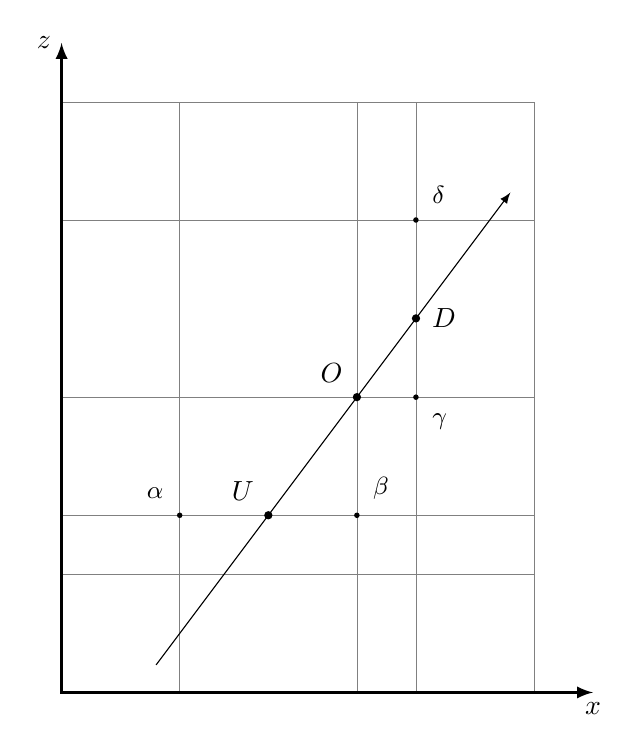
\begin{tikzpicture}[scale=1.5, line width=1pt, >=latex]
    \def\xcoords{1,2,3.5,4,5}
    \def\xmax{5}
    \def\ycoords{1,2,2.5,3.5,5,6}
    \def\ymax{6}
    \def\raym{4/3}
    \def\rayc{-7/6}

    \draw [help lines]
    \foreach \y in \ycoords {
        (1, \y) -- (\xmax, \y)
    }
    \foreach \x in \xcoords {
        (\x, 1) -- (\x, \ymax)
    };
    \draw [<->] ({\xmax+0.5}, 1) node[below] {$x$} -- (1,1) -- (1, {\ymax+0.5}) node[left] {$z$};
    \coordinate (O) at (3.5, 3.5);
    \node[circle, fill=black, inner sep=0 pt, minimum size=3pt, label=above left:{$O$}] at (O) {};
    \draw[->, domain=1.8:4.8, samples=10, thin] plot(\x, {\raym * (\x) + \rayc});
    \coordinate (D) at (4, {\raym * 4 + \rayc});
    \node[circle, fill=black, inner sep=0 pt, minimum size=3pt, label=right:{$D$}] at (D) {};
    \coordinate (U) at ({(2.5 - \rayc) / (\raym)}, 2.5);
    \node[circle, fill=black, inner sep=0 pt, minimum size=3pt, label=above left:{$U$}] at (U) {};

    \node[circle, fill=black, inner sep=0 pt, minimum size=2pt, label={[label distance=0.5mm]above left:{\small $\alpha$}}] at (2, 2.5) {};
    \node[circle, fill=black, inner sep=0 pt, minimum size=2pt, label={[label distance=0.5mm]above right:{\small $\beta$}}] at (3.5, 2.5) {};
    \node[circle, fill=black, inner sep=0 pt, minimum size=2pt, label={[label distance=0.5mm]below right:{\small $\gamma$}}] at (4, 3.5) {};
    \node[circle, fill=black, inner sep=0 pt, minimum size=2pt, label={[label distance=0.5mm]above right:{\small $\delta$}}] at (4, 5) {};
\end{tikzpicture}
\caption{Diagram of short characteristics scheme in two-dimensions.}
\label{Fig:Sc2d}
\end{figure}

For each ray prescribed by the angular quadrature the formal solver must perform one sweep through the grid.
The general case, that of an inclined ray ray travelling through the atmosphere is shown in, Fig.~\ref{Fig:Sc2d}.
In the case of this ray the formal solver must sweep first along $x$ and then along $z$.
The points $U$ and $D$ refer to them being ``upwind'' and ``downwind'' of the point $O$ for which we are currently computing the intensity.
This can be explained by looking at the intersections of ray with the grid.
To compute the intensity in the direction of this ray at point $O$ using the short characteristics formulation we have
\begin{equation}
   I_O = I_U e^{-(\tau_U - \tau_O)} + \int_{\tau_O}^{\tau_U} S(t) e^{-(t - \tau_O)}\, dt,
\end{equation}
where these terms have their usual meanings, $I_O$ is the intensity in this direction at $O$, $I_U$ is the intensity in this direction at $U$ and we have dropped the angular and frequency dependencies for clarity.
Thus, to compute the intensity at $O$, the intensity at $U$ must first be known.
As $U$ does not typically lie on a point of our discrete two-dimensional grid, the value of $I_U$ (and other quantities) are not computed directly by the formal solver, and must instead be interpolated from the values of grid points along the line $\alpha\beta$.

Following the short characteristic method, a functional form must be assigned to the variation of $S$ over the the line segment $[UO]$.
In the simplest case, this can again be a linear functional form, but due to the additional axis for inhomogeneities that can be present in the two-dimensional case, unless the grid is very fine or the atmosphere very slowly varying, this may be a poor choice.
A higher order parametrisation of $S$ is likely to require the values of the source function at both $U$ and $D$, and possibly other points along this path.
Similarly to the cubic Bézier spline method used as standard in our plane-parallel code, we once again turn to monotonic Bézier splines for safe, smooth interpolation, minimising the presence of under and over-shoots.
The cubic method we apply in plane-parallel atmospheres requires four points along $UD$, which becomes less practical in higher dimensions, due to the large computational demands of the method.
Instead we choose the quadratic Bézier spline method, BESSER, of \citet{Stepan2013}, which will be briefly summarised here for the scalar case of the RTE.
The BESSER method differs from other quadratic Bézier spline methods by ensuring the continuity of the first derivative of the interpolant at $O$.
Due to the large differences in optical depth between adjacent regions (e.g. $\tau_{UO}$ and $\tau_{OD}$) that are likely to occur in multi-dimensional cases with irregular grids, this method is designed so as to guarantee that if values over $[UOD]$ are monotonic then the spline interpolant will remain monotonic.


% \begin{figure}
% \centering
% \begin{tikzpicture}[scale=1.5, line width=1pt, >=latex]
%     \def\xcoords{1,2,3.5,4,5}
%     \def\xmax{5}
%     \def\ycoords{1,2,2.5,3.5,5,6}
%     \def\ymax{6}
%     \def\raym{0.6}
%     \pgfmathsetmacro\rayc{3.5 - \raym * 3.5}

%     \draw [help lines]
%     \foreach \y in \ycoords {
%         (1, \y) -- (\xmax, \y)
%     }
%     \foreach \x in \xcoords {
%         (\x, 1) -- (\x, \ymax)
%     };
%     \draw [<->] ({\xmax+0.5}, 1) node[below] {$x$} -- (1,1) -- (1, {\ymax+0.5}) node[left] {$z$};
%     \coordinate (O) at (3.5, 3.5);
%     \node[circle, fill=black, inner sep=0 pt, minimum size=3pt, label=above left:{$O$}] at (O) {};
%     \draw[->, domain=1.2:4.8, samples=10, thin] plot(\x, {\raym * (\x) + \rayc});
%     \coordinate (D) at (4, {\raym * 4 + \rayc});
%     \node[circle, fill=black, inner sep=0 pt, minimum size=3pt, label=right:{$D$}] at (D) {};
%     \coordinate (U) at ({(2.5 - \rayc) / (\raym)}, 2.5);
%     \node[circle, fill=black, inner sep=0 pt, minimum size=3pt, label=above left:{$U$}] at (U) {};

%     \node[circle, fill=black, inner sep=0 pt, minimum size=2pt, label={[label distance=0.5mm]above left:{\small $\alpha$}}] at (2, 2.5) {};
%     \node[circle, fill=black, inner sep=0 pt, minimum size=2pt, label={[label distance=0.5mm]above right:{\small $\beta$}}] at (3.5, 2.5) {};
%     \node[circle, fill=black, inner sep=0 pt, minimum size=2pt, label={[label distance=0.5mm]below right:{\small $\gamma$}}] at (4, 3.5) {};
%     \node[circle, fill=black, inner sep=0 pt, minimum size=2pt, label={[label distance=0.5mm]above right:{\small $\delta$}}] at (4, 5) {};
% \end{tikzpicture}
% \caption{Diagram of Short Characteristics Scheme in 2D}
% \label{Fig:Sc2d}
% \end{figure}

{\color{TolBlue} do the explanation/diagrams; boundary conditions!, vertical case}

{\color{Red} Need to cite linear, parabolic (Auer 94?), BESSER (stepan2013) Ibgui substepping}

\subsection{Implementation Details}

From this description of the process, it is clear that there is a more complex ordering in which the atmospheric points must be visited than in the plane-parallel case (which can only be top--bottom or vice-versa).
In the case of a single-threaded program, it is sufficient to obey this order, however, when distributing work across threads or multiple computing nodes it is essential that the necessary information be present to avoid computation stalls, or the use of uninitialsed data.
There is an in-depth discussion of an advanced parallelisation algorithm for multi-dimensional radiative transfer in \citet{Stepan2013}, however in \Lw{} we assume that the entire simulation domain can be held in memory and the formal solver is parallelised in frequency, equivalently to the plane-parallel case.

The data structures for storing the atmospheric and population information in \Lw{} were also updated to support two dimensional atmospheres, storing the data contiguously so as to be able to reuse the core iteration machinery from the plane-parallel case (as inspired by the RH code).
Two-dimensional formal solvers can be loaded from external libraries via the same interface as used for their one-dimensional counterparts, and through these interfaces we ensure the modularity of \Lw{}.
An equivalent interface is also defined for the iteration function to be used in two-dimensions, giving flexibility in the interpolation order and any form of limiting used (which may need to be adapted to specific grids).
\Lw{} provides default implementations of the two-dimensional linear and BESSER short-characteristics formal solvers, along with linear and WENO4 interpolation schemes.

{\color{Red} Do we want a validation test here; can do in place.}